\chapter{PROPOSTA}
\label{Proposta}

Este capítulo apresenta a descrição da proposta do trabalho, introduzindo ferramentas e técnicas que auxiliam no desenvolvimento de aplicações para Internet, disponibilizando \textit{code patterns} que podem ser praticados a fim de manter um código único para toda a equipe, tornando a manutenção facilitada e evitando conflitos de sintaxe e formatação. A organização por seções inicia-se em~\ref{CodePattern}, onde são abordadas técnicas de padronização de código bem como a utilização de \textit{plug-ins} para facilitar a escrita de código. Por fim, em~\ref{Otimizacao}, são descritas técnicas visando a otimização da aplicação.

\section{Padrão de Estilo de Código}
\label{CodePattern}

Atualmente, existem diversos \textit{plug-ins} disponíveis para garantir uma escrita padronizada de código, também conhecida por \textit{style code pattern}. Neste trabalho, opta-se pela utilização de determinados \textit{plug-ins} de código fonte aberto devido à sua popularidade com a comunidade de desenvolvedores, indicada pelo número de contribuidores ativos, além de suas documentações mais abrangentes e acessíveis. Estes podem ser utilizados para tornar o desenvolvimento mais padronizado, retirando a responsabilidade do desenvolvedor a garantia de um código limpo. Desta forma, o programador é capaz de se responsabilizar principalmente pelas regras de negócio, pois com o auxílio destes \textit{plug-ins}, a padronização é realizada de forma automatizada.

\subsection{Babel}
\label{SubBabel}

Conversor de código e responsável por transpor códigos escritos de uma determinada sintaxe para outra, podendo também minimizar código removendo os comentários e espaçamentos desnecessários (\textit{stripped}). Além disso, o Babel é capaz de renomear variáveis e objetos para uma escrita ilegível por humanos (\textit{uglify}) em meio ao processo de conversão.

A grande maioria dos navegadores não implementa o padrão ES6 por completo, disponibilizando apenas o suporte oficial completo com a versão ES5 e pequenas \textit{features} da versão mais recente. Com Babel é possível escrever o código inteiramente em uma versão mais moderna e obter um arquivo de código gerado em uma versão totalmente compatível com os navegadores mais antigos. Isso, torna mais fácil o processo de migração para o desenvolvedor, que pode escrever código de próximas gerações sem se preocupar com a compatibilidade e mantendo foco apenas no desenvolvimento.
%
%
%
\subsection{ESLint}
\label{SubESLint}

Como pode-se observar na Tabela~\ref{tab:eslintvsjshint}, recomenda-se a utilização do ESLint devido sua popularidade com a comunidade de desenvolvedores, além de sua vasta documentação~\footnote{ESLint é um utilitário de \textit{linting} plugável para JavaScript. Seu guia de uso está disponível em: https://eslint.org/docs/user-guide/; Acesso realizado em 9 de Abril de 2018.}. Além do ESLint, existem outros \textit{plug-ins}, tal como o JSHint, que realizam tarefas similares. Todavia, além de realizar verificação léxica e sintática, o ESLint permite personalizar regras para erros, e oferece suporte completo ao ES6.

\begin{table}[th]
\centering
\caption{Comparativo entre ESLint e JSHint.}
\label{tab:eslintvsjshint}
\begin{tabular}{llll}
                &   ESLint  &   JSHint\\\hline

Favoritos       &   11.056  &   7.905\\
\textit{Forks}  &   1.906   &   1.646\\
Contribuidores  &   599     &   235\\
Licença         &   MIT     &   MIT\\
Criação         &   06/2013 &   11/2010\\
\hline
\end{tabular}
\begin{flushleft}
\flushleft{Fonte: Repositórios Oficiais no GitHub. Data de Acesso: 10 de Abril de 2018.}
\end{flushleft}
\end{table}

A função do ESLint neste conjunto com o Babel é a de garantir a padronização do código, sendo configurado em um arquivo~\texttt{.eslintrc} para delimitar espaçamento, nomenclatura e até comentários, o que torna um código mais rígido e consequentemente único. Suas regras de configuração garantem o uso de boas práticas proibindo a utilização de determinados artifícios de linguagem e aconselhando a utilização de outros, por exemplo: a utilização obrigatória de identidade~"==="~ao invés de simples igualdade~"=="~a fim de garantir o mesmo valor e tipo de dado. Como o JavaScript não é uma linguagem compilada, os erros são observados em tempo de execução. Com o auxílio do ESLint, é possível perceber um futuro erro antes mesmo do código ser interpretado. No entanto, outros \textit{plug-ins} podem complementar esta tarefa.
%
%
%
\subsection{Prettier}
\label{SubPrettier}

Formatador de código para IDE, o \textit{Prettier} embeleza o código utilizando as regras estabelecidas no ESLint (Subseção~\ref{SubESLint}). Este \textit{plug-in} analisa as regras de escrita de código e o padrão adotado, por exemplo: standardjs; AirBnb; dentre outros. Ele permite também que, ao salvar alterações no arquivo, o código seja formatado automaticamente. Isso torna o desenvolvimento mais rápido e contribui para a diminuição de erros. A extensão oferece suporte para os seguintes editores e IDEs: Sublime Text; Atom; VS Code; dentre outros. Além disso, ele é compatível com as sintaxes: ES6; JSON; Vue; CSS3+; SCSS e derivados.
%
%
%
\subsection{PostCSS}
\label{SubPostCSS}

Assim como o JavaScript, o CSS também possui ferramentas desenvolvidas para oferecer uma gama maior de recursos não disponíveis na versão oficial ou suportados pelos navegadores atuais, como o PostCSS. Aliada a esta justificativa, existe a garantia de compatibilidade \textit{cross-browser} provida pela ferramenta utilizada, que converte a linguagem estendida em linguagem de estilo em cascata nativa.

Existem diversas soluções de pré-processadores CSS, tais como SASS, LESS e Stylus. Estas ferramentas utilizam sintaxe própria, baseada ou compatível completamente com CSS, que implementam recursos avançados a fim de tornar o código mais reutilizável e o desenvolvimento mais ágil. A problemática destes pré-processadores se resume na forma com que implementam suas soluções, muitas vezes amarrando o desenvolvimento e gerando uma incompatibilidade entre pré-processadores. Devido as suas peculiaridades, torna-se, no mínimo, trabalhoso migrar um código escrito originalmente em LESS para Stylus por exemplo. 

PostCSS é a solução mais versátil e minimalista, além de ser o projeto mais popular em número de colaboradores. Segundo a Tabela~\ref{tab:postcss}, pode-se ver um maior destaque de sua aceitação, além de ser o projeto mais recente. PostCSS também é modular, o que torna possível a instalação de diversos \textit{plug-ins} para a resolução de problemas ou simplesmente por uma instalação limpa. A sua modularidade permite com que o desenvolvedor não seja responsável pela compatibilidade entre navegadores, mas tenha poder de escolher como é executada a solução. É possível, através do \textit{plug-in}~\texttt{cssnext}, escrever CSS de ultima geração sem se preocupar com os navegadores que ainda não implementaram as novas especificações de sintaxe. Também existem outros \textit{plug-ins} específicos para cada necessidade, tais como:
\begin{itemize}
    \item \texttt{autoprefixer}~\textemdash~Adiciona prefixos específicos de navegador às regras CSS, baseado nos valores disponíveis no Can I Use~\footnote{O \textit{Can I Use} (https://caniuse.com/) é uma importante base de dados online que disponibiliza consulta sobre a implementação de regras CSS nos diversos navegadores existentes. Acesso em: 10 de Abril de 2018.}.
    \item \texttt{css-modules}~\textemdash~Remove a necessidade de escrever classes com nomes extensos, basta utilizar o mais genérico, este módulo evita, automaticamente, conflitos em escopos de módulos distintos.
    \item \texttt{stylelint}~\textemdash~A melhor solução para evitar erros de sintaxe em sua folha de estilos.
    \item \texttt{lost}~\textemdash~O \textit{LostGrid} faz uso da função CSS~\texttt{calc()}~para criar grades impressionantes baseadas em frações que são definidas com configuração mínima.
\end{itemize}

\begin{table}[th]
\centering
\caption{Comparativo entre Pré-Processadores CSS e PostCSS.}
\label{tab:postcss}
\begin{tabular}{llll}
                &   SASS    &   LESS        &   PostCSS\\\hline

Favoritos       &   11.256  &   15.460      &   18.112\\
\textit{Forks}  &   1.976   &   3.465       &   990\\
Contribuidores  &   186     &   216         &   249\\
Licença         &   MIT     &   Apache-2.0  &   MIT\\
Criação         &   06/2006 &   02/2010     &   09/2013\\
\hline
\end{tabular}
\begin{flushleft}
\flushleft{Fonte: Repositórios Oficiais no GitHub. Data de Acesso: 10 de Abril de 2018.}
\end{flushleft}
\end{table}

PostCSS é um parser de CSS, desenvolvido em JavaScript, capaz de criar uma árvore sintática abstrata e depois transformar isso em CSS novamente através de quatro etapas de atuação, que são:
\begin{itemize}
    \item \textbf{Análise Léxica}~\textemdash~O código CSS passa por um processo de \textit{tokenization}. Neste processo, são descartados caracteres como espaços extra, indentação e quebras de linha.
    \item \textbf{Criação da Árvore}~\textemdash~Um algoritmo capaz de processar o \textit{array} de \textit{tokens} e criar uma estrutura em árvore. Relacionando valores à propriedades, propriedades à seletores, seletores à \textit{media queries} e etc.
    \item \textbf{Uso de \textit{Plug-ins}}~\textemdash~A árvore criada no passo anterior é passada sequencialmente por uma lista de \textit{plug-ins}, sofrendo alterações no caminho.
    \item \textbf{Retorno}~\textemdash~É de responsabilidade do \textit{stringifier}; um algoritmo que recebe a árvore modificada e a transforma novamente em CSS.
\end{itemize}

É importante perceber que o PostCSS em instalação limpa não adiciona variáveis, \textit{mixins}, \textit{partials} ou quaisquer dessas funcionalidades. Tampouco especifica uma nova sintaxe. Se algo é uma alternativa aos pré-processadores conhecidos, são os \textit{plug-ins}. Sem eles, o PostCSS apenas lê o CSS e reescrevê-lo exatamente como ele o encontrou. Os \textit{plug-ins} são os responsáveis por todas as funcionalidades. E esse é o ponto mais importante desse novo ecossistema de processamento de CSS: A responsabilidade, a governança, e o mesmo código não estão centralizados em um único projeto.
%
%
%
\subsection{Webpack}
\label{SubWebpack}

O \textit{Webpack} é um empacotador de módulos (\textit{bundler}). Seu principal objetivo é agregar arquivos JavaScript para uso em navegador, mas também é capaz de transformar, empacotar ou anexar qualquer recurso ou ativo.

Além de arquivos JavaScript, através da utilização de \textit{plug-in}, pode-se configurar o \textit{Webpack} para modularizar código, executar funções do Babel (Subseção~\ref{SubBabel}), comprimir imagens, realizar funções de rotina e até iniciar um servidor HTTP para o desenvolvimento da aplicação. \textit{Webpack} é responsável por realizar o \textit{build} e gerar arquivos estáticos. Ele lista as dependências e gera um gráfico de dependência, permitindo que os desenvolvedores utilizem uma abordagem modular para seus propósitos de desenvolvimento. O \textit{bundler} pode ser configurado usando um arquivo de configuração externo chamado~\texttt{webpack.config.js}~ou pode ser usado a partir da linha de comando.
%
%
%
\subsection{Git}
\label{SubGit}

Git é um sistema de controle de versão distribuído e um sistema de gerenciamento de código fonte, com ênfase em velocidade. Bastante recomendado para o desenvolvimento de aplicações, principalmente quando há mais de um indivíduo envolvido na criação de código.

Não necessariamente contribui diretamente para a construção de código padronizado como sugere a Seção~\ref{CodePattern}, porém permite uma gerência de código para a equipe, versionando e armazenando um histórico de alterações. Ou seja, ele fornece recursos indispensáveis para o desenvolvimento compartilhado de uma aplicação moderna. Por estas razões, Git localiza-se nesta seção, sendo categorizado como uma boa prática.
%
%
%
%
%
%
%
%
%
\section{Técnicas para Otimização}
\label{Otimizacao}

Juntamente com a utilização de diversos \textit{plug-ins} para o desenvolvimento ágil de aplicações \textit{Web} modernas, técnicas podem ser aplicadas a fim de obter-se o máximo de eficiência em ambiente de produção tornando a experiência de execução para o usuário mais fluida e leve.

\subsection{Tela de Abertura}
\label{SubSplashScreen}

\textit{Splash Screen} é uma técnica bastante utilizada em aplicações compiladas que consiste em exibir uma imagem ou animação de carregamento enquanto o binário é carregado, passando a impressão ao usuário que a aplicação já está sendo carregada quando na verdade, muitas vezes, o processo já está sendo executado e algum recurso ainda não está pronto. Em aplicações \textit{Web} também é possível criar telas de abertura.

Para aplicar a técnica em um ambiente \textit{Web}, antes é necessário entender como funciona o carregamento de uma página bem como o funcionamento básico do DOM, citado na fundamentação teórica na Subseção~\ref{SubNavegador}, onde o navegador é descrito. Os navegadores baixam o HTML e o CSS do servidor e depois analisam e adicionam as \textit{tags} HTML aos nós do DOM, criando uma árvore chamada árvore de conteúdo. Este processo consiste de três fases que são:
\begin{itemize}
    \item \textbf{Fase 1}~\textemdash~Enquanto o HTML é analisado, o motor de renderização cria uma nova árvore chamada de árvore de renderização. Esta árvore representa os efeitos visuais com os quais os elementos serão exibidos.
    \item \textbf{Fase 2}~\textemdash~Após os processos acima, ambas as árvores passam pelo processo de \textit{layout}, onde o navegador posiciona na área do documento cada nó (elemento). Isto é chamado pelo W3C de esquema de posicionamento, que instrui o navegador onde e como cada elemento deverá ser inserido, conforme três tipos: fluxo normal, \textit{floaters} e posição absoluta.
    \item \textbf{Fase 3}~\textemdash~A fase final chamada \textit{painting} (pintura). É o processo gradual onde o motor de renderização percorre a árvore de renderização aplicando todos os efeitos visuais, como tamanhos, cores etc. Esta fase pode ser observada quando se abre uma página em uma conexão mais lenta, podendo ver os estilos visuais sendo aplicados conforme a página é renderizada.
\end{itemize}

Como visto no item 3 (\textit{painting}) da lista acima, na fase de pintura, a árvore de renderização é atravessada e o método de \textit{painting} dos renderizadores é solicitado para exibir seu conteúdo na tela. A pintura utiliza o componente de infraestrutura da interface do usuário. É neste momento que deve ser exibido o conteúdo da página. Como é desejada uma tela de abertura, há a necessidade de se tardar o \textit{script} principal para a tela durar determinado tempo previamente determinado ou simplesmente exibir primariamente a animação de carregamento e ocultar esta animação quando o conteúdo for completamente carregado, fazendo com que a página imprima um conteúdo visual estático antes de haver um conteúdo interativo.

O JavaScript dispõe de diferentes janelas de tempo que acontecem durante o carregamento de página. Essas janelas de tempo são delineadas pelos eventos \texttt{DOMContentLoaded} e \texttt{OnLoad}. O primeiro acontece quando a árvore DOM encontra-se pronta e disponível para manipulação. Já o último, é liberado apenas quando todo o conteúdo é carregado, bem como os estilos e as imagens. É no evento de~\texttt{OnLoad}~que a página não realiza mais requisição de conteúdo inicial, isto é, aquele indicador de carregamento na aba do navegador é finalizado.
%
%
%
\subsection{Critical CSS}
\label{SubCriticalCSS}

Esta técnica consiste em carregar apenas o conteúdo crítico ao estilo da página, desta forma, é reduzido o tempo para a visualização inicial, tornando uma experiência mais fluida e um carregamento mais rápido ao diminuir a quantidade de código carregado. Sendo assim, o CSS crítico é carregado primeiro e em seguida o não crítico.

Quando as dependências de um documento HTML são carregadas, há um bloqueio de renderização "\textit{render-blocking}", que significa que o navegador não pode exibir a página até que o recurso seja baixado ou tratado de outra forma. Quando esta página é carregada por um navegador da \textit{Web}, ela é lida de cima para baixo. Quando o navegador chegar à \textit{tag}~\texttt{<link>}, ele começa a baixar a folha de estilos imediatamente e não renderiza a página até que ela seja concluída. Quanto maior o tamanho do arquivo a ser carregado, maior o tempo de espera do usuário até que a transferência e leitura sejam realizadas. Mas não significa que um bloqueio de renderização seja algo ruim, somente deve-se saber utilizá-lo. Caso a folha de estilo não seja carregada no cabeçalho do documento, mas em seu corpo, acontece uma anomalia que pode ser visualizada na Figura~\ref{fig:withoutcss}~chamada de \textit{"flash of unstyled content"}.

\begin{figure}[th]
\centering{
\caption{\textit{Flash} de conteúdo não estilizado.}
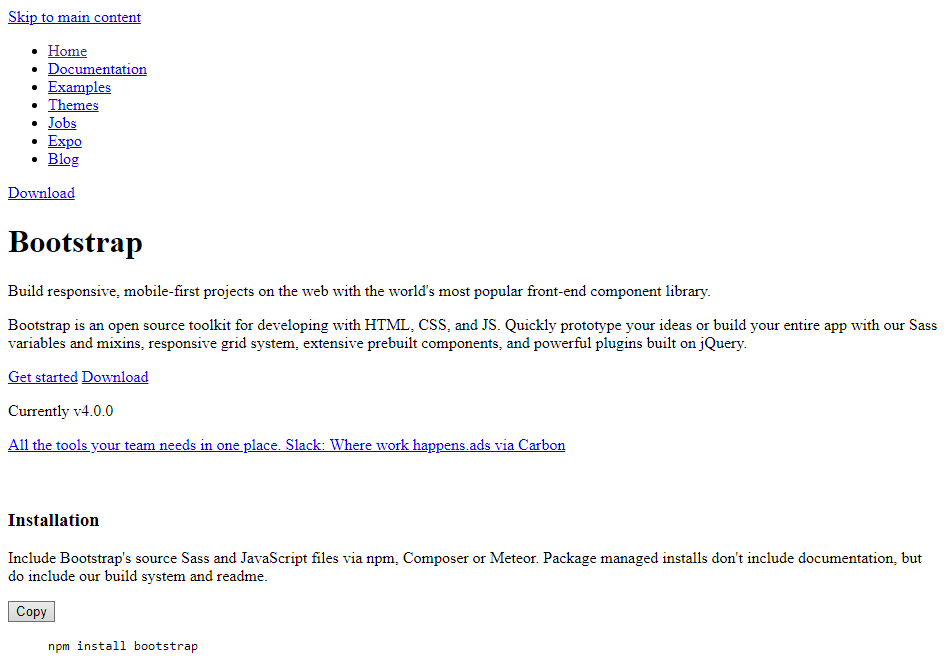
\includegraphics[width=0.75\textwidth]{figuras/withoutcss}
\begin{flushleft}
\flushleft{Fonte: Site do Bootstrap. Acesso em 9 de Abril de 2018.}
\end{flushleft}
\label{fig:withoutcss}
}
\end{figure}

O ponto ideal que queremos é onde renderizar a página com o CSS crítico necessário para estilizar a visualização principal, mas todo o CSS não crítico é carregado após a renderização inicial. Na Figura~\ref{fig:withcss} pode ser observada a aparência que deveria ser apresentada após o carregamento inicial de página.

\begin{figure}[th]
\centering{
\caption{Aparência Inicial Esperada.}

\includegraphics[width=0.75\textwidth]{figuras/withcss}
\begin{flushleft}
\flushleft{Fonte: Site do Bootstrap. Acesso em 9 de Abril de 2018.}
\end{flushleft}
\label{fig:withcss}
}
\end{figure}

Determinados componentes visuais, considerados críticos, devem aparecer de prontidão bem como suas regras de estilo. Todavia, componentes secundários que não representam impacto para a visualização inicial do documento não são necessários para a exibição imediata. Tendo isto em mente, é necessário isolar o CSS crítico do CSS não crítico. Para isto, são criadas duas folhas de estilo:~\texttt{critical.css} e \texttt{non\_critical.css}, que separam os estilos crítico do não-crítico, respectivamente. Suas importações podem ser realizadas através do elemento \texttt{<link>}, juntamente com \texttt{<script>} ou arquivo externo contendo JavaScript.

\begin{lstlisting}[label=criticalcss,caption=CSS Crítico.]
<!DOCTYPE html>
<html lang="pt-br">
    <head>
        <meta charset="utf-8">
        <title>Monografia</title>
        <link rel="stylesheet" href="critical.css">
    </head>
    <body>
        <script>
            require("non_critical.css");
        </script>
    </body>
</html>
\end{lstlisting}

O trecho de Código~\ref{criticalcss}, escrito em ES6 para fins didáticos, ilustra como acontece a importação de uma folha de estilos em cascata crítica. Através do cabeçalho do documento e um arquivo não crítico, importado por meio de código JavaScript no corpo do arquivo HTML. Estas duas importações fazem com que o arquivo crítico seja lido inicialmente, no momento que a página é carregada e, posteriormente, quando a árvore DOM estiver montada no documento. Sendo assim, quando o arquivo de \textit{script} for lido, o restante do estilo CSS é carregado junto ao documento também. É importante mencionar que o exemplo acima não funciona em navegadores atuais e, sua versão em ES5 foi omitida devido à grande extensão de linhas de código.

Como visto na Subseção~\ref{SubWebpack}, o \textit{Webpack} é responsável por resolver programaticamente diversas atividades. Ele pode ser útil com o auxílio de alguns \textit{plug-ins} para a identificação do CSS crítico automaticamente, visto que identificar manualmente pode ser uma tarefa árdua e repetitiva ao longo do período de desenvolvimento. Um destes \textit{plug-ins} é o~\texttt{critical}, disponível no NPM~\footnote{\textit{Node Package Manager} (NPM) é o maior gerenciador de pacotes para JavaScript, disponível em: https://www.npmjs.com/. Data de acesso: 10 de Abril de 2018.}. Este módulo em JavaScript é responsável pela leitura de um documento HTML, para, posteriormente identificar o CSS crítico através de uma renderização de página no servidor. Para isso, é utilizado o PhantomJS~\footnote{Phantom JS é um \textit{headless browser}, ou seja, um navegador que não renderiza as páginas. Ele apenas executa o código que está contido nas páginas, tornando-o uma ferramenta comum para um ambiente de integração contínua.}, outro módulo JavaScript disponível no NPM, que, por sua vez, extraias regras CSS aplicadas na página então renderizada pelo servidor com PhantomJS.

É importante ressaltar que esta solução descrita acima foi idealizada com base no cenário atual sob o protocolo HTTP/1.1, disponível na Subseção~\ref{SubHTTP}. Com o avanço do protocolo e a promessa de suportar multiplexação, o ideal é realizar requisições e respostas assíncronas e paralelas utilizando apenas uma conexão para baixar múltiplos arquivos. Isso pode fazer com que, através do protocolo HTTP/2 ou superior, seja possível obter primordialmente o código CSS crítico em uma modificação da técnica atual, através do uso da multiplexação em conjunto com \textit{Critical} CSS.

No Capítulo~\ref{Resultados}, são apresentados os resultados deste experimento. Com o intuito de validar a otimização em questão, espera-se obter um retorno satisfatório com base nas métricas utilizadas na execução do teste. Além disso, contém as descrições dos resultados dos experimentos.
%
%
%
\subsection{Reduzir o \textit{Payload}}
\label{SubPayload}

Em aplicações para rede de computadores e, principalmente voltadas para \textit{Web}, é inevitável deparar-se com o \textit{payload}~\footnote{\textit{Payload} refere-se à carga de uma transmissão de dados.}. Uma boa prática de desenvolvimento para aplicações \textit{Web} é tentar reduzir este volume de dados, uma vez que dados trafegam pela \textit{Web} entre aplicações distribuídas. Para isso, há diversas técnicas que podem ser utilizadas para reduzir o \textit{payload}.

Uma dessas técnicas é reduzir o número de requisições. Desenvolver serviços para Internet, pensando em baixas velocidades de conexão, bem como aplicando a estratégia do \textit{mobile first}~\footnote{\textit{Mobile First} é uma estratégia de desenvolvimento contrária ao histórico modelo de desenvolvimento de aplicações \textit{Web}, onde a versão móvel era tratada de forma secundária.}, são boas práticas para o desenvolvimento de aplicações \textit{Web}. Determinadas requisições podem ser irrelevantes por completo ou apresentar conteúdo parcialmente desnecessário. Por exemplo, ao realizar uma requisição HTTP com o verbo GET, os dados retornados são: \texttt{id}; \texttt{name}; \texttt{birthday}; \texttt{address}. Sendo que, esta requisição será utilizada apenas para popular um \texttt{<select>} que, por sua vez, necessita apenas de um atributo \texttt{value}, referenciando o valor selecionado de uma opção com um texto indicativo. Os dados necessários para popular este elemento HTML podem ser resumidos a dois: \texttt{id} e o dado exibido. Por exemplo, uma lista de usuários necessitaria de \texttt{id}~e~\texttt{name}, apenas.

Outra técnica comum, é o agrupamento de arquivos do mesmo tipo, como arquivos de \textit{script} e folhas de estilo, por exemplo. Apesar de aumentar o \textit{payload}, com a transferência de um arquivo único de \textit{bundle}, composto do agrupamento de todos os arquivos JavaScript, cujo o tamanho é a soma de todos os tamanhos dos arquivos aglomerados. A perda no aumento do \textit{payload} é compensada devido ao comportamento atual do protocolo HTTP/1.1, onde não há multiplexação e as requisições são síncronas, ou seja, um arquivo é enviado após o outro. As respostas, no melhor caso, retornam para o cliente com o mesmo custo de tempo de envio de um único arquivo aglomerado. Entretanto, podem ocorrer complicações em rede, tais como: Falha na entrega de um dos arquivos, causado pela perda de pacotes; Atraso na Rede, devido à latência ou congestionamento de fluxo; dentre outros problemas comuns em redes de computadores. Sendo assim, justifica-se a criação de um arquivo composto da união de vários outros para o envio.

Há também outro artificio que consiste em habilitar a compressão GZIP~\footnote{GZIP é um formato de compactação de arquivos, identificado pela extensão~\texttt{.gz}. Descrito na RFC 1952 por \citeonline{rfc1952}.}~no servidor. Esta técnica é suportada em todos os navegadores e servidores contemporâneos. Com o processo de compactação, todo o conteúdo textual (i.e. HTML, CSS, JS, etc) é comprimido antes de ser enviado para o cliente, contribuindo assim, para a diminuição do tráfego total em rede.

Em conjunto com a agregação de arquivos e redução do número de requisições, é importante também, comprimir os códigos gerados. Isto é, não basta escrever JavaScript elegante, bem documentado, organizado e padronizado. Estas características são agradáveis para se manter e manutenir, porém o navegador não entende linguagem humana não se importa com a organização do código. Enviar código padronizado via requisição HTTP para o lado cliente não acrescentará valor algum à performance do código. Para isto que deve-se utilizar um compressor de arquivos, por exemplo o módulo~\texttt{uglify-js}, disponível no NPM. Após agregar todos os \textit{scrips} em um único, tecnicamente, não há nada além de uma simples concatenação em um novo arquivo de \textit{script}. Com uma ferramenta de otimização, como o~\texttt{uglify-js}, o código agregado é processado e comprimido, a fim de diminuir o tamanho do arquivo gerado como saída. Neste processo, também chamado de \textit{minification}, os espaçamentos são removidos, assim como a indentação, a nomenclatura dos objetos e variáveis é renomeada para uma versão minificada baseada em escopo. Em outras palavras, uma variável chamada de~\texttt{option}~pode ser renomeada para apenas~\texttt{o}~e suas correspondentes dentro do escopo da função seguem o mesmo processo de maneira que não haja conflitos. Todo esse processo é realizado automaticamente e o resultado produz um arquivo de agregação comprimido e ilegível para linguagem humana, apresentando um menor número de caracteres.

Imagens também podem ser otimizadas, no formato~\texttt{.jpeg}, há uma série de metadados desnecessários. E no formato~\texttt{.png}, as paletas de cores são definidas, porém, também não são necessárias. Estas informações extra consomem alguns KB de memória a mais, que não representam importância para sua reprodução no cliente. Além desta otimização, é importante utilizar os atributos~\texttt{width}~e~\texttt{height}~para contribuir com os cálculos de dimensões realizados pelo navegador durante a renderização de página. Entretanto, não devem ser utilizados os mesmos atributos para redimensionar o tamanho das imagens importadas, devem ser declarados os tamanhos reais. Por exemplo, se uma imagem nas dimensões~\texttt{50px}~por~\texttt{50px}~for exibida, não deve-se importar uma imagem de tamanho superior e compensar a proporção com os atributos~\texttt{width}~e~\texttt{height}. O custo desta prática será a importação de uma imagem de tamanho superior e que não é utilizada, recomenda-se otimizar, também, a imagem em seu tamanho.